\section{Evaluation}\label{sec:eval}
We evaluate the proposed approach for the following research questions:
\begin{itemize}
\item RQ1. (Correctness) Does the transformation correctly distribute the
  training of single-GPU models?
\item RQ2. (Effectiveness) Does the automated transformation effectively accelerate the
  training of single-GPU models?
\end{itemize}

\noindent
To answer the questions, we implemented an automatic code transformation tool
and applied the tool to 16 TensorFlow DL models.
We collected the evaluation target models from five open repositories: 
Hovorod\cite{horovodgithub}, TensorFlow Model Garden\cite{tfmodelgarden},
TensorFlow Examples by Americ Damien\cite{tfexamplesdamien},
CIFAR-10 Example with TensorFlow 2.0\cite{cifar10github}, and
TensorFlow 2.x Tutorials\cite{tf2tutogithub}.
We excluded two from 18 models in the repositories because one abnormally
terminates with a runtime error in its execution, and the other duplicates.
Our tool is written in Scala and is publicly
available\footnote{https://github.com/kaist-plrg/python-analyzer}.

\begin{table}[!ht]
  \begin{center}
  \caption{Experiment result for the automated code transformation}
  \label{fig:eval:targets}
  \begin{tabular}{l|c|c|c}
    \hline
    \multicolumn{1}{c|}{Source} & Model Name & API Pattern & Transform Result\\
    \hline\hline
    TensorFlow Examples by &  LSTM-MNIST & GradientTape & $\bigcirc$\\
     Americ Damien\cite{tfexamplesdamien} & SimpleCNN-GradientTape-1 & GradientTape & $\times$\\
    \hline
    \multirow{2}{*}{Horovod GitHub\cite{horovodgithub}} & SimpleCNN-GradientTape-2 & GradientTape & $\bigcirc$\\
    & SimpleCNN-MonitoredSession & MonitoredSession  & $\bigcirc$\\
    \hline
    TensorFlow Model Garden\cite{tfmodelgarden} & SimpleCNN-Session & Session & $\bigcirc$\\ 
    \hline
    \hspace{-.5em}\begin{tabular}{l}
      CIFAR-10 Example with\\ TensorFlow 2.0\cite{cifar10github}
    \end{tabular}& VGG-CIFAR10 & Keras & $\bigcirc$\\ 
    \hline
    \multirow{10}{*}{TensorFlow 2.x Tutorials\cite{tf2tutogithub}} & Play-with-MNIST & GradientTape & $\bigcirc$\\
    &Linear-Regression & GradientTape & $\bigcirc$\\
    &Fashion-MNIST & Keras  & $\bigcirc$\\
    &CIFAR10-VGG16 & GradientTape & $\bigcirc$\\
    &Inception-Network & GradientTape  & $\bigcirc$\\
    &RNN-Sentiment-Analysis & Keras  & $\bigcirc$\\
    &Stacked-LSTM-ColorBot & GradientTape  & $\bigcirc$\\
    &Auto-Encoder & GradientTape  &$\bigcirc$\\
    &Variational-Auto-Encoder & GradientTape & $\bigcirc$\\
    &DCGAN & GradientTape & $\bigcirc$\\ 
    \hline
  \end{tabular}
  \end{center}
%  \caption{List of the TensorFlow DL models used for the experiments}
\end{table}
%%%%%%%%%%%%%%%%%%%%%%%%%%%%
%\pagebreak
%\begin{figure}[!ht]
%  \begin{center}
%  \begin{tabular}{c|c|l}
%    \hline
%    Model Name & API Pattern & Source \\
%    \hline
%    LSTM-MNIST & GradientTape & \multirow{2}{*}{TensorFlow Examples by Americ Damien\cite{tfexamplesdamien}} \\
%    SimpleCNN-GradientTape-1 & GradientTape \\
%    \hline
%    SimpleCNN-GradientTape-2 & GradientTape & \multirow{2}{*}{Horovod GitHub\cite{horovodgithub}} \\
%    SimpleCNN-MonitoredSession & MonitoredSession  \\
%    \hline
%    SimpleCNN-Session & Session & TensorFlow Model Garden\cite{tfmodelgarden} \\
%    \hline
%    VGG-CIFAR10 & Keras & CIFAR-10 Example with TensorFlow 2.0\cite{cifar10github} \\
%    \hline
%    Play-with-MNIST & GradientTape & \multirow{10}{*}{TensorFlow 2.x Tutorials\cite{tf2tutogithub}} \\
%    Linear-Regression & GradientTape  \\
%    Fashion-MNIST & Keras  \\
%    CIFAR10-VGG16 & GradientTape \\
%    Inception-Network & GradientTape  \\
%    RNN-Sentiment-Analysis & Keras  \\
%    Stacked-LSTM-ColorBot & GradientTape  \\
%    Auto-Encoder & GradientTape  \\
%    Variational-Auto-Encoder & GradientTape  \\
%    DCGAN & GradientTape  \\
%    \hline
%  \end{tabular}
%  \end{center}
%  \caption{List of the TensorFlow DL models used for the experiments}
%  \label{fig:eval:targets}
%\end{figure}


\subsection{RQ1: Correctness of the transformation}
To show the correctness of the transformation, we transformed each of the 16
single-GPU models using our tools and compared them to the distributed training
versions of those models.
For the models obtained from the Horovod repository, we used their distributed
training versions available in the repository as the correct results.
As for the other models, we referred to the Horovod documentation to manually
transform them into distributed training versions and used those as the correct
results.

%To answer the first research question,
%we conducted a transformation experiment.
%The transformation experiment evaluates whether the transformation tool
%correctly transforms single-GPU based models to distributed models.
%We specify the correctness of transfomation by pairing each model codes 
%with hand-crafted code of the distributed versions. 
%The models from the Horovod GitHub repository\cite{horovodgithub}
%come with corresponding distributed versions.
%For other models that do not come with distributed versions,
%we manually crafted their distributed implmentations.

%\begin{figure}[!ht]
%  \begin{center}
%  \begin{tabular}{|c|c|c|}
%    \hline
%    Model Name & API Pattern & Transformation Success \\
%    \hline
%    LSTM-MNIST & GradientTape & o \\
%    SimpleCNN-GradientTape-1 & GradientTape & x\\
%    SimpleCNN-GradientTape-2 & GradientTape & o \\
%    SimpleCNN-MonitoredSession & MonitoredSession &o\\
%    SimpleCNN-Session & Session & o\\
%    VGG-CIFAR10 & Keras & o \\ 
%    Play-with-MNIST & GradientTape & o \\
%    Linear-Regression & GradientTape & o \\
%    Fashion-MNIST & Keras & o \\
%    CIFAR10-VGG16 & GradientTape & o\\
%    Inception-Network & GradientTape & o \\
%    RNN-Sentiment-Analysis & Keras & o \\
%    Stacked-LSTM-ColorBot & GradientTape & o \\
%    Auto-Encoder & GradientTape & o \\
%    Variational-Auto-Encoder & GradientTape & o \\
%    DCGAN & GradientTape & o \\
%    \hline
%  \end{tabular}
%  \end{center}
%  \caption{Transformation experiment Result}
%  \label{fig:eval:trans}
%\end{figure}

\begin{figure}[!ht]
  \begin{lstlisting}[language=Python]
# Model object is not used, instead a function used
def conv_net(x):
    x = tf.reshape(x, [-1, 28, 28, 1])
    conv1 = conv2d(x, weights['wc1'], biases['bc1'])
    conv1 = maxpool2d(conv1, k=2)
    conv2 = conv2d(conv1, weights['wc2'], biases['bc2'])
    conv2 = maxpool2d(conv2, k=2)
    fc1 = tf.reshape(conv2, [-1, weights['wd1'].get_shape().as_list()[0]])
    fc1 = tf.add(tf.matmul(fc1, weights['wd1']), biases['bd1'])
    fc1 = tf.nn.relu(fc1)
    out = tf.add(tf.matmul(fc1, weights['out']), biases['out'])
    return tf.nn.softmax(out)

optimizer = tf.optimizers.Adam(learning_rate)

def run_optimization(x, y):
    with tf.GradientTape() as g:
        pred = conv_net(x)
        loss = cross_entropy(pred, y) 
    trainable_variables = list(weights.values()) + list(biases.values())
    gradients = g.gradient(loss, trainable_variables)
    optimizer.apply_gradients(zip(gradients, trainable_variables))
    # cannot perform variable broadcast with Model.variables

# training loop
for step, (batch_x, batch_y) in enumerate(train_data.take(training_steps), 1):
    run_optimization(batch_x, batch_y)\end{lstlisting}
  \caption{Training code of SimpleCNN-GradientTape-1 model}
  \label{fig:eval:simplecnn1}
\end{figure}


Table~\ref{fig:eval:targets} represents the transformation experiment results.
The first column shows the repositories from which obtaining the models, the
second column shows the model names, the third column shows the API patterns of
the models, and the fourth column shows whether our tool correctly transforms
the models.
As shown in the table, our tool correctly transformed 15 out of the 16 models
and failed to transform only the SimpleCNN-GradientTape-1 model.
In the failed case, our tool raised a transformation failure error because
some of the GradientTape transformation rules do not apply to the model.


%The transformation experiment result is described in the 
%figure \ref{fig:eval:trans}. Among 16 targets, only one model failed to
%be correctly transformed. As shown in the figure \ref{fig:eval:trans},
%the SimpleCNN-GradientTape-1 model failed to be transformed into the
%distributed model.

We manually investigated the SimpleCNN-GradientTape-1 model code to 
identify the cause of the transformation failure.
Figure~\ref{fig:eval:simplecnn1} illustrates the training code snippet of the
model.
The code uses a GradientTape object in lines 17 to 22 to train a model
constructed via a sequence of TensorFlow API calls in lines 3 to 12.
As described in Section~\ref{sec:grad}, our approach transforms the
GradientTape pattern code by injecting statements that broadcast trainable
variables of a {\tt Model} instance.
However, because the code does not construct the model as a {\tt Model}
instance, our tool cannot obtain the trainable variables from the model and
fails to transform the code correctly.
Note that such model construction is rare because our tool correctly transforms
11 out of the 12 GradientTape models since they utilize a {\tt Model}
instance.


\subsection{RQ2: Effectiveness of the automatically distributed training}
For the second research question, we conducted a comparative analysis
between the training time of the automatically transformed models and their
respective original models.
We calculate the training time as the time taken to reach minimum losses in
training.
To measure the losses, we manually injected the TensorBoard\cite{tensorboard}
API calls into the model codes, which log the loss value of each training
epoch.
Among the 16 models, we targeted 13 models in the experiment; we excluded two
TensorFlow 1.x models with which the TensorBoard APIs are incompatible 
and one that our tool failed to transform.
We experimented on a Linux machine with Intel Xeon CPU E5-2690 v4 @
2.60GHz, 131GB memory, and four NVIDIA TITAN Xp GPUs.

%To answer the second research question,
%we conducted a distributed training experiment that compares
%the training speed between the original models
%and corresponding transform models.
%To quantify the training speed, we measured the epoch loss during the training
%of each model.
%Among 16 models used for the first experiment,
%we excluded two TensorFlow 1.x models (SimpleCNN-MonitoredSession,
%SimpleCNN-Session) and the SimpleCNN-GradientTape-1 model that failed to
%correctly be transformed.
%Thus, we targeted total 13 models for the distributed training experiment.
%We manually added the TensorBoard\cite{tensorboard} APIs to 
%record the loss value during the training. 
%The experiment server uses
%Intel Xeon CPU E5-2690 v4 @ 2.60GHz with 131GB memory and four 
%NVIDIA TITAN Xp GPUs.



\begin{table}
  \centering
  \caption{Training time comparison results}
  \label{fig:eval:traintime}
  \begin{tabular}{|l|r|r|r|}
\hline
                         & Single-GPU         & Distributed       & \\
Model Name               &  training time (s) & training time (s) &  Speedup\\
\hline
LSTM-MNIST               & 78.675& 11.951& $\times$6.58\\
SimpleCNN-GradientTape-2 & 3.192& 1.753& $\times$1.82\\
VGG-CIFAR10              & 967.076 & 299.229 &$\times$3.23\\
Play-with-MNIST          & 148.101& 80.040& $\times$1.85\\
Linear-Regression        & 0.607& 0.371& $\times$1.63\\
Fashion-MNIST            & 110.274& 29.294& $\times$3.76\\
CIFAR10-VGG16            & 1060.296& 1159.293& $\times$0.91\\
Inception-network        & 956.261& 995.597& $\times$0.96\\
RNN-Sentiment-Analysis   & 338.984& 451.985& $\times$0.74\\
Stacked-LSTM-ColorBot    & 57.327 & -           & -   \\
Auto-Encoder             & 567.230& 412.214& $\times$1.37\\
Variational-Auto-Encoder & 1120.291& 699.777& $\times$1.60\\
DCGAN                    & 2389.052& 828.428& $\times$2.88\\ 
\hline
  \end{tabular}
\end{table}

We summarize the training time comparison results in
Table~\ref{fig:eval:traintime}.
The first column presents the model name, the second and third columns
present the training time of the model, and the last column presents the
training speed-up of the distributed model.
The comparison results indicate that the training of the distributed
models is, on average, approximately 2.28 times faster than that of the
original models; when distributed training has a positive effect on the
training time, the enhancement ranges from 1.37 times to 6.58 times.
Note that we do not record the distributed training time of the
Stacked-LSTM-ColorBot model because the loss of the first distributed training
epoch of the model is minimal.

\begin{figure}%[!ht]
  \centering
  \begin{subfigure}[t]{.24\textwidth}
    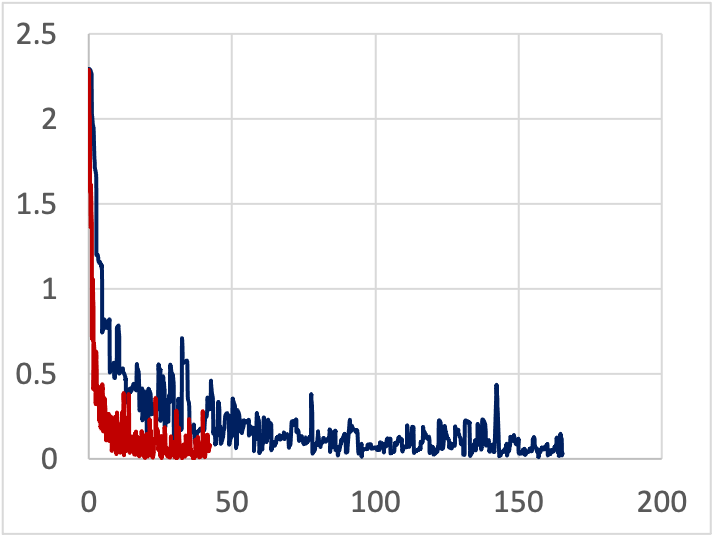
\includegraphics[width=\textwidth]{tape-lstm}
    \caption{LSTM-MNIST}
  \end{subfigure}
  ~ 
  \begin{subfigure}[t]{.36\textwidth}\centering
    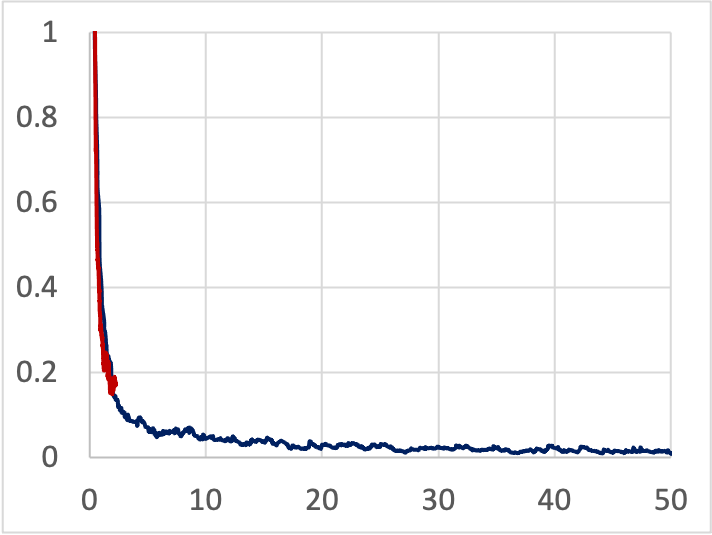
\includegraphics[width=.66\textwidth]{tape-simple2}
    \caption{SimpleCNN-GradientTape-2}
  \end{subfigure}
  ~
  \begin{subfigure}[t]{.24\textwidth}
    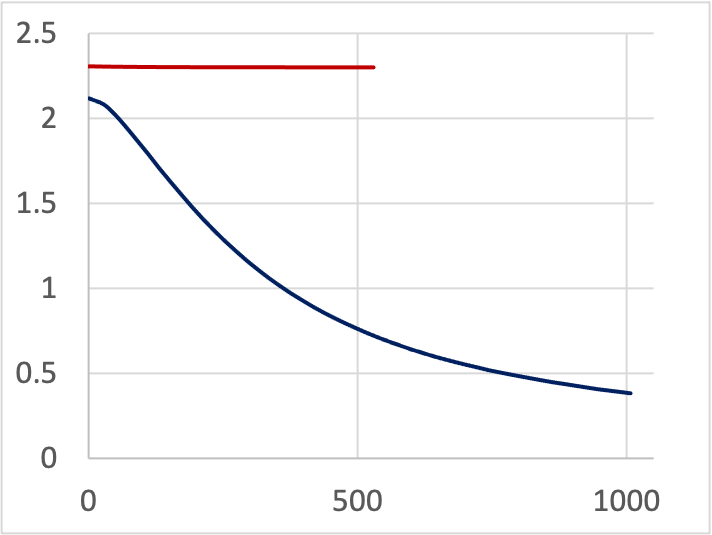
\includegraphics[width=\textwidth]{keras-cifar}
    \caption{VGG-CIFAR10}
  \end{subfigure}
  \par\bigskip
  \begin{subfigure}[t]{.24\textwidth}
    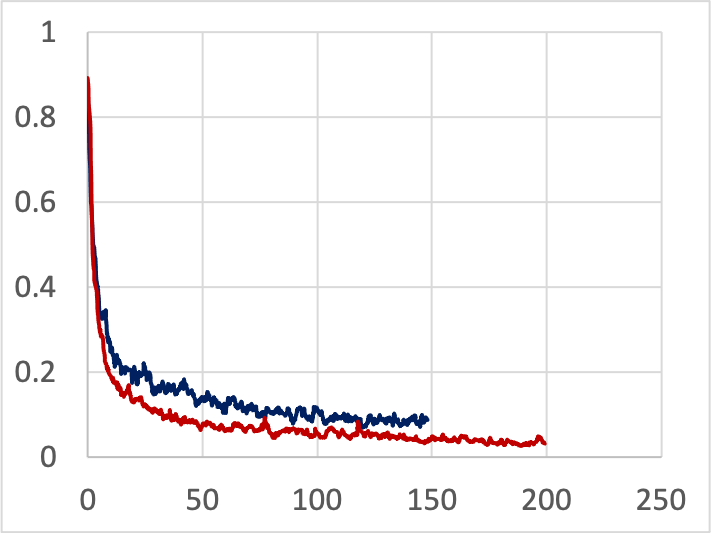
\includegraphics[width=\textwidth]{tf2-03}
    \caption{Play-with-MNIST}
  \end{subfigure}
  ~
  \begin{subfigure}[t]{.24\textwidth}
    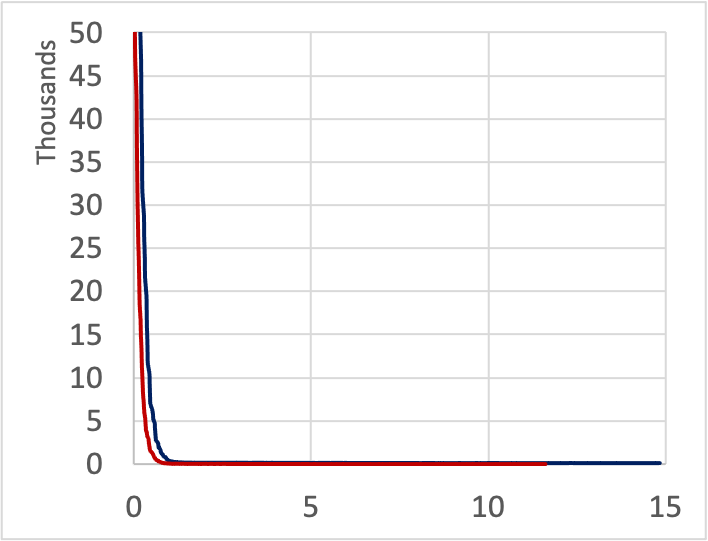
\includegraphics[width=\textwidth]{tf2-04}
    \caption{Linear-Regression}
  \end{subfigure} 
  ~ 
  \begin{subfigure}[t]{.24\textwidth}
    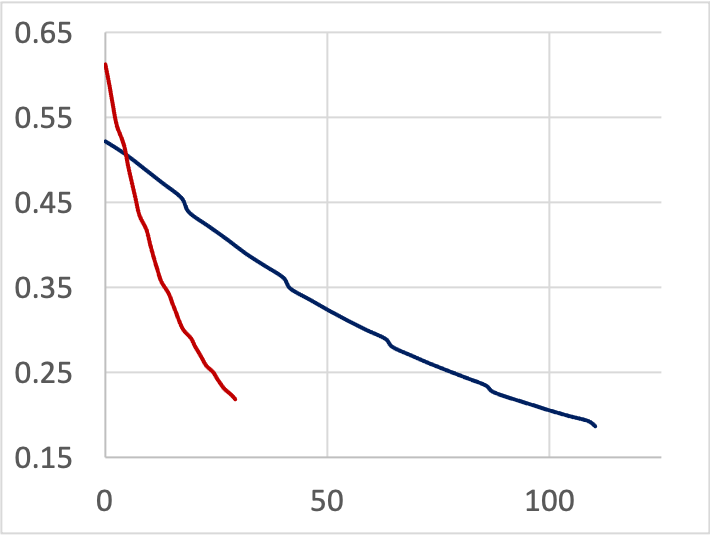
\includegraphics[width=\textwidth]{tf2-05}
    \caption{Fashion-MNIST}
  \end{subfigure}
  ~
  \begin{subfigure}[t]{.24\textwidth}
    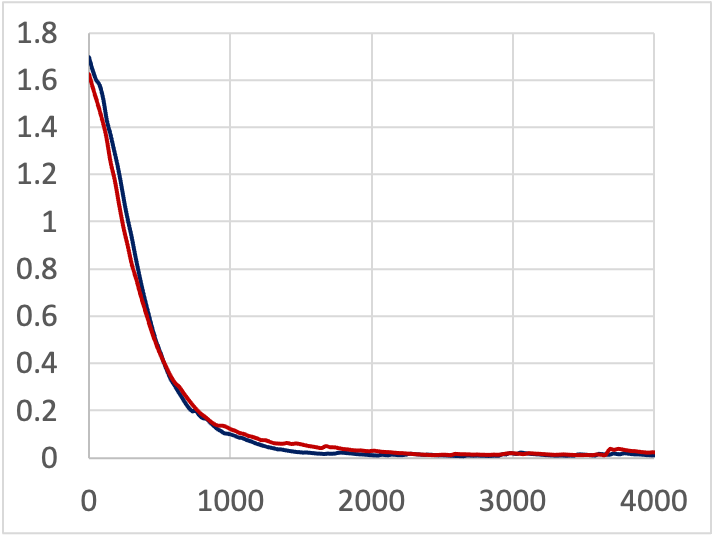
\includegraphics[width=\textwidth]{tf2-06}
    \caption{CIFAR10-VGG16}
  \end{subfigure}
  \par\bigskip
  \begin{subfigure}[t]{.24\textwidth}
    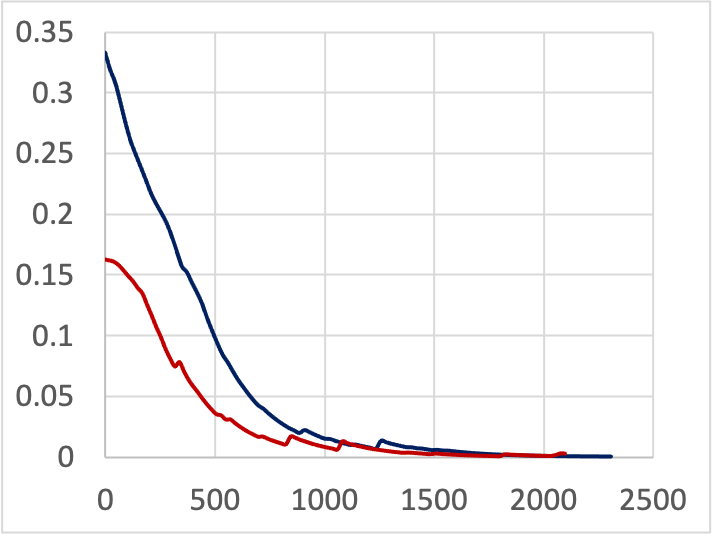
\includegraphics[width=\textwidth]{tf2-07}
    \caption{Inception-network}
  \end{subfigure}
  ~
  \begin{subfigure}[t]{.24\textwidth}
    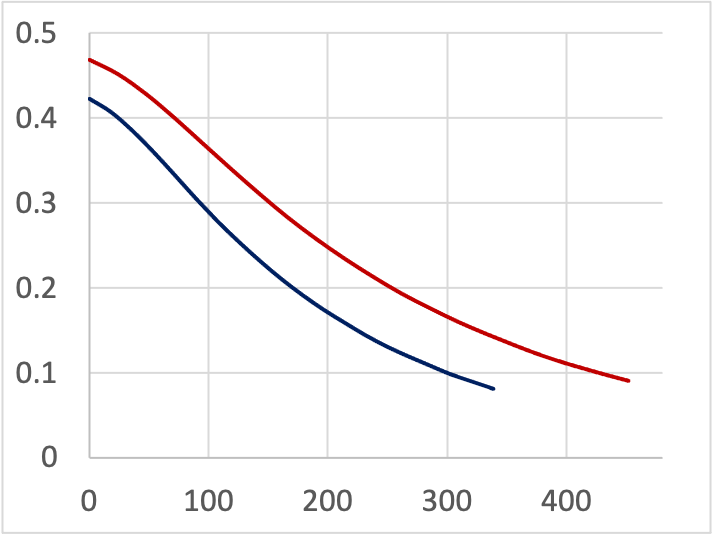
\includegraphics[width=\textwidth]{tf2-09}
    \caption{RNN-Sentiment-Analysis}
  \end{subfigure} 
  ~ 
  \begin{subfigure}[t]{.24\textwidth}
    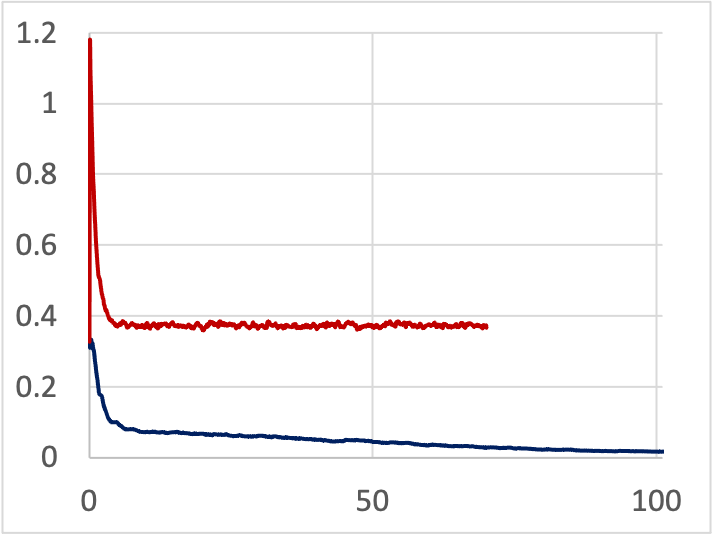
\includegraphics[width=\textwidth]{tf2-10}
    \caption{Stacked-LSTM-ColorBot}
  \end{subfigure}
  ~
  \begin{subfigure}[t]{.24\textwidth}
    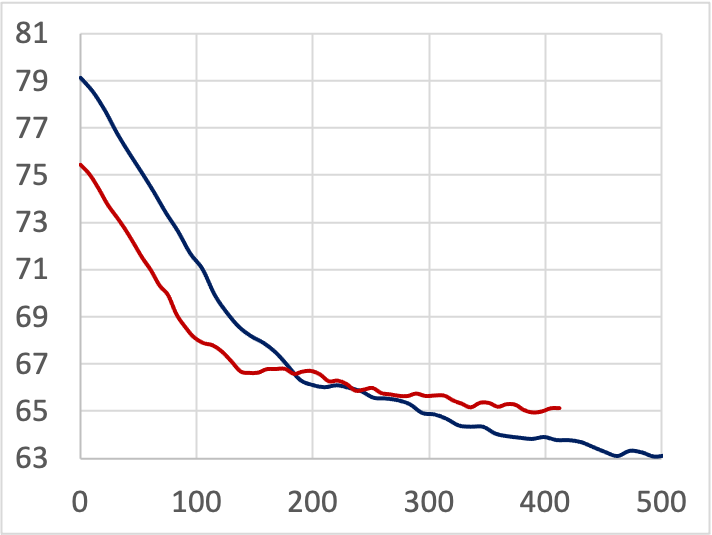
\includegraphics[width=\textwidth]{tf2-11}
    \caption{Auto-Encoder}
  \end{subfigure}
  \par\bigskip
  \begin{subfigure}[t]{.24\textwidth}
    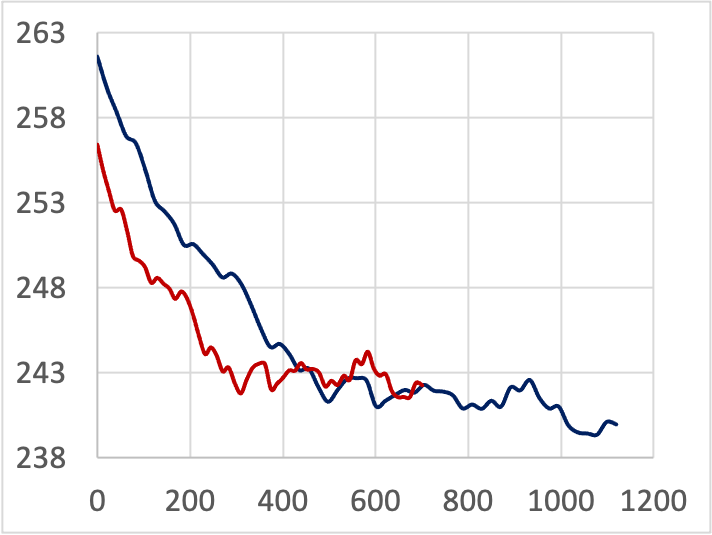
\includegraphics[width=\textwidth]{tf2-12}
    \caption{Variational-Auto-Encoder}
  \end{subfigure}
  ~
  \begin{subfigure}[t]{.24\textwidth}
    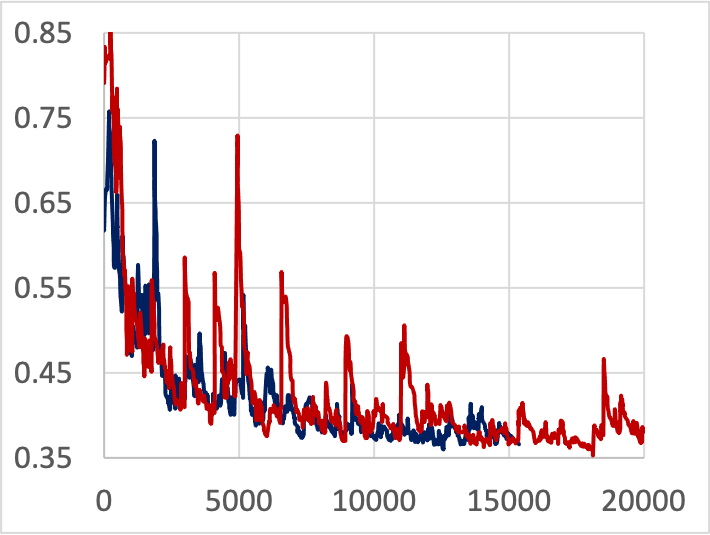
\includegraphics[width=\textwidth]{tf2-13}
    \caption{DCGAN}
  \end{subfigure} 

  \caption{Comparison of training between the distributed models and the
  original models (X-axis: time in seconds, Y-axis: loss value, blue-line:
  original model, red-line: distributed model)}
  %\begin{tabular}{r@{: }l r@{: }l}
  %  X-axis & Time (seconds) & Y-axis & Loss value\\
  %  Blue line & ORG loss, smoothed & Red line & HVD loss, smoothed\\ 
  %\end{tabular}
  \label{fig:eval:train}
\end{figure}

Interestingly, distributed training does not ensure an acceleration of
training.
In three models, distributed training takes longer to reach
minimum losses than non-distributed training.
Furthermore, distributed training can harm the inference precision of models.
Figure~\ref{fig:eval:train} illustrates the changes in the loss of models over
training time. 
The x-axis represents the training time in seconds, the y-axis represents the
loss values, and the blue and red lines represent the losses of the
original models and their transformed models, respectively.
Distributed training in six models led to higher losses than
non-distributed training.
For instance, in the case of the VGG-CIFAR10 model, we observed that the loss
gradually decreases during the training process without distributed training.
However, when adopting distributed training, the loss did not decrease
significantly and remained almost unchanged, with only minor fluctuations.

%The results of the distributed traininig experiment 
%are shown in figure \ref{fig:eval:train} and figure \ref{fig:eval:traintime}.
%Figure \ref{fig:eval:train} graphically describes the change of training loss
%of single GPU-based models and distributed models over time.
%The x-axis represent the time in seconds, and the y-axis represent
%the loss value number.
%The lines represent the loss values;
%blue lines correspond to the single GPU-based model training loss
%and the red lines correspond to the distributed model training loss.
%Figure \ref{fig:eval:traintime} show the training times required in
%single GPU-based models and distributed models.
%To define the training time, we first calculated the total reduction of
%loss by finding the maximum and minimum losses.
%We define that the training has completed when the loss decreased by
%95\% of the loss reduction amount, and the time up to that point
%was defined as the training time.
%The fourth column of figure \ref{fig:eval:traintime} 
%shows the relative speedup of the 
%distributed model training with respect to the single GPU-based model training.
%Note that the Stacked-LSTM-ColorBot model does not have distributed training
%time recorded. This is because the loss values after the first epoch
%are always higher that the initial loss value; thus the training time is
%undefined.

%As shown in the results in figure \ref{fig:eval:traintime},
%only 8 out of 13 distributed models show speedup. 
%Figure \ref{fig:eval:train} also shows that some models are erroneously trained.
%In figure \ref{fig:eval:train}(c), the distributed training of
%VGG-CIFAR10 model does not decrease the loss value.
%In figure \ref{fig:eval:train}(j), the distributed training of
%Stacked-LSTM-ColorBot model increases the loss value.
%In general, the experiment result implies that even if the transformation
%of the model code is successful, it does not guarantee
%increase in the training speed of the distributed models.

Distributed training often requires additional tuning of hyperparameters to
achieve positive effects.
We conducted distributed training on the VGG-CIFAR10 model by applying three
different learning rate parameters.
Figure~\ref{fig:eval:cifar10} shows the experiment result.
The gray line represents the result of non-distributed training, the red line
represents the result of distributed training with the original learning rate
of $1e-3$, and the blue and black lines represent the results of distributed
training with adjusted learning rates of $1e-4$ and $1e-5$, respectively.
The three distributed training cases reached the minimum loss nearly
simultaneously but exhibited significant differences in the
achieved minimum loss for each training.
In the case of distributed training with the original learning rate, the
training led to only slight changes in loss.
However, when adjusting the learning rate to $1e-4$ in distributed training, 
we observed that the minimum loss significantly decreased to a similar level
to that of non-distributed training.
In the case of distributed training with the learning rate adjusted to $1e-5$,
the result for the minimum loss was better than distributed training with the
original learning rate but worse than non-distributed training.
This experiment shows that model engineers may need to tune hyperparameters
differently from non-distributed models to obtain the benefits of distributed
training.

\begin{figure}%[!ht]
  \centering
  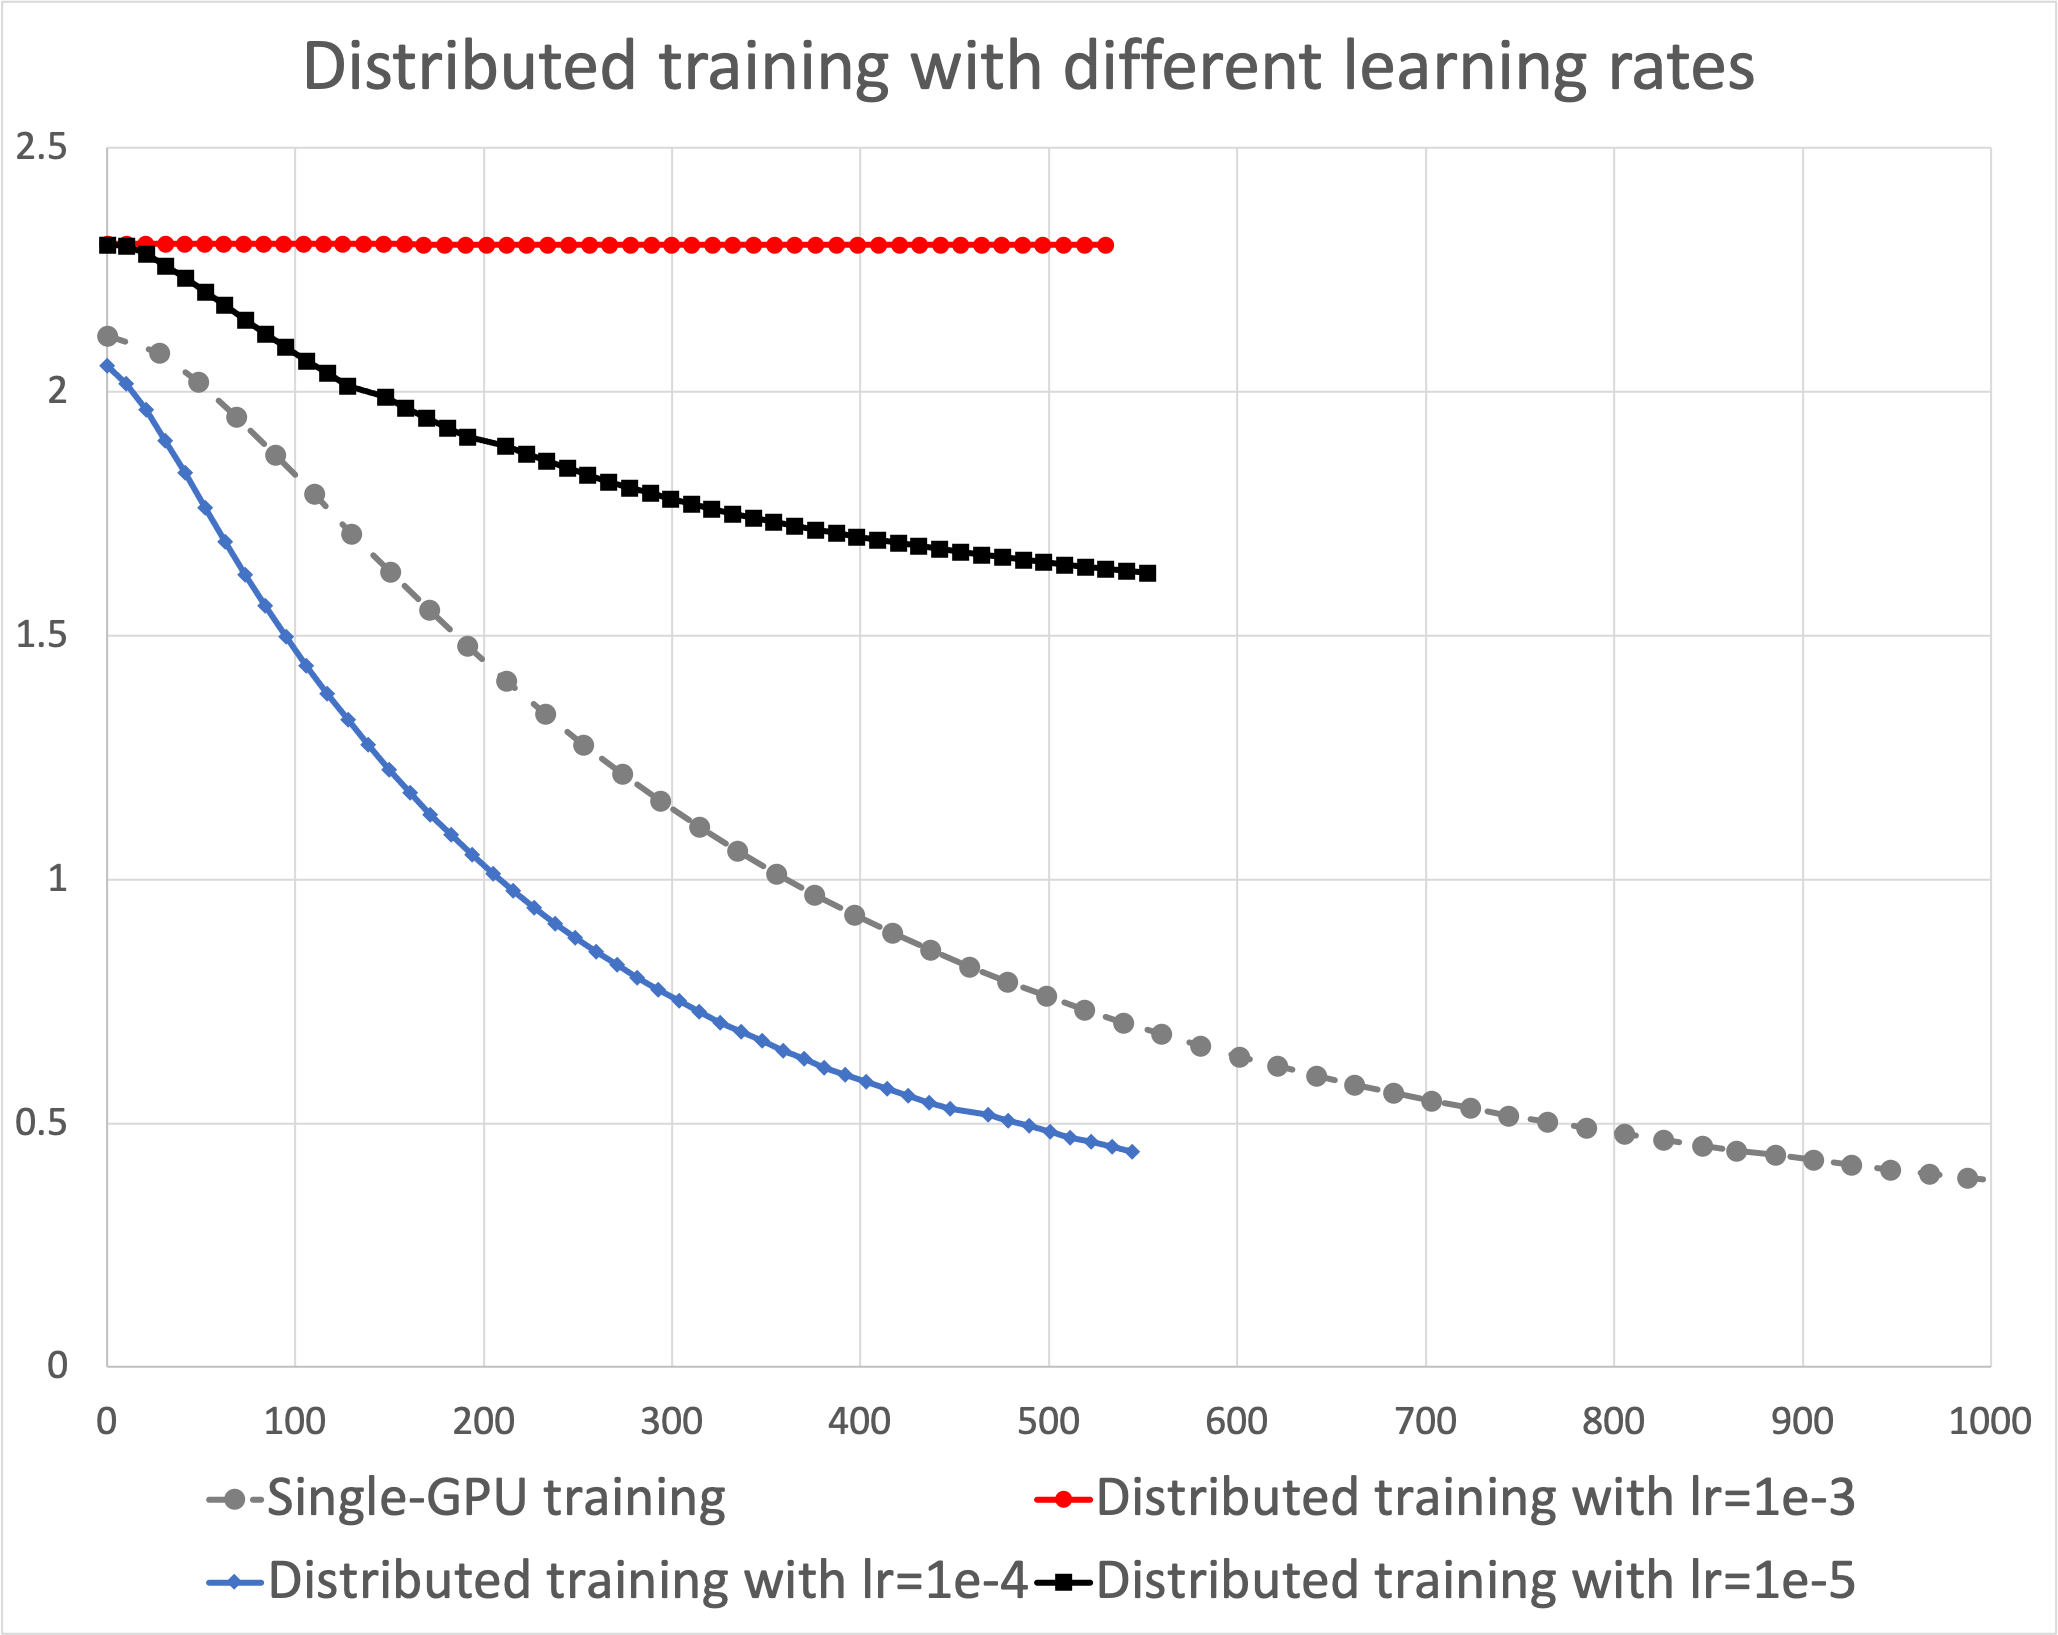
\includegraphics[width=.5\textwidth]{lr-exp-graph}
  \caption{Distributed training on the VGG-CIFAR10 model with different learning rates}
  \label{fig:eval:cifar10}
\end{figure}

%We claim that training hyperparameters can be tuned to
%achieve the distributed training speedup.
%We provide an experimental evidence to this by
%training the distributed VGG-CIFAR10 model with
%different learning rates.
%Learning rate value of the original VGG-CIFAR10 model is 0.001,
%We altered this value to 0.0001, 0.00001
%and compared the training loss changes over time.

%Figure \ref{fig:eval:cifar10} shows the loss value changes of training 
%distributed VGG-CIFAR10 models with different learning rates.
%The distributed training with the original learning rate=0.001 does not show
%training speedup.
%However, when the learning rate is changed to 0.0001,
%the distributed training shows speedup compared to the single GPU training.
%Changing the learning rate to 0.00001 does not increases training speed
%compared to the single GPU training, but its speed is higher than
%the distributed training with the original learnin rate.
%By this experiment, we show that tuning the learning rate into right place 
%increases the distributed training speed.  

%Our automated transformation approach reduces much friction and time between
%writing single GPU-based model and deploying the model in distributed system.
%The transformation tool quickly transforms the single GPU-based
%models into the distributed model and initiate the training process.
%Using the transformation tool, the model engineers can start the distributed
%training process without effort to rewrite the model codes. 
%Our transformation tool requires users to manually inspect the
%training speed and tune the hyperparameters.
%This is the minimal amount of effort which is always required for
%scaling and distributing DL models.
